\subsection{Wichtige Beispiele \formelbuch{204ff}} %Seitenzahlen OK 10 Auflage
	\subsubsection{Ellipse {\formelbuch{205}}} %Seitenzahlen OK 10 Auflage
		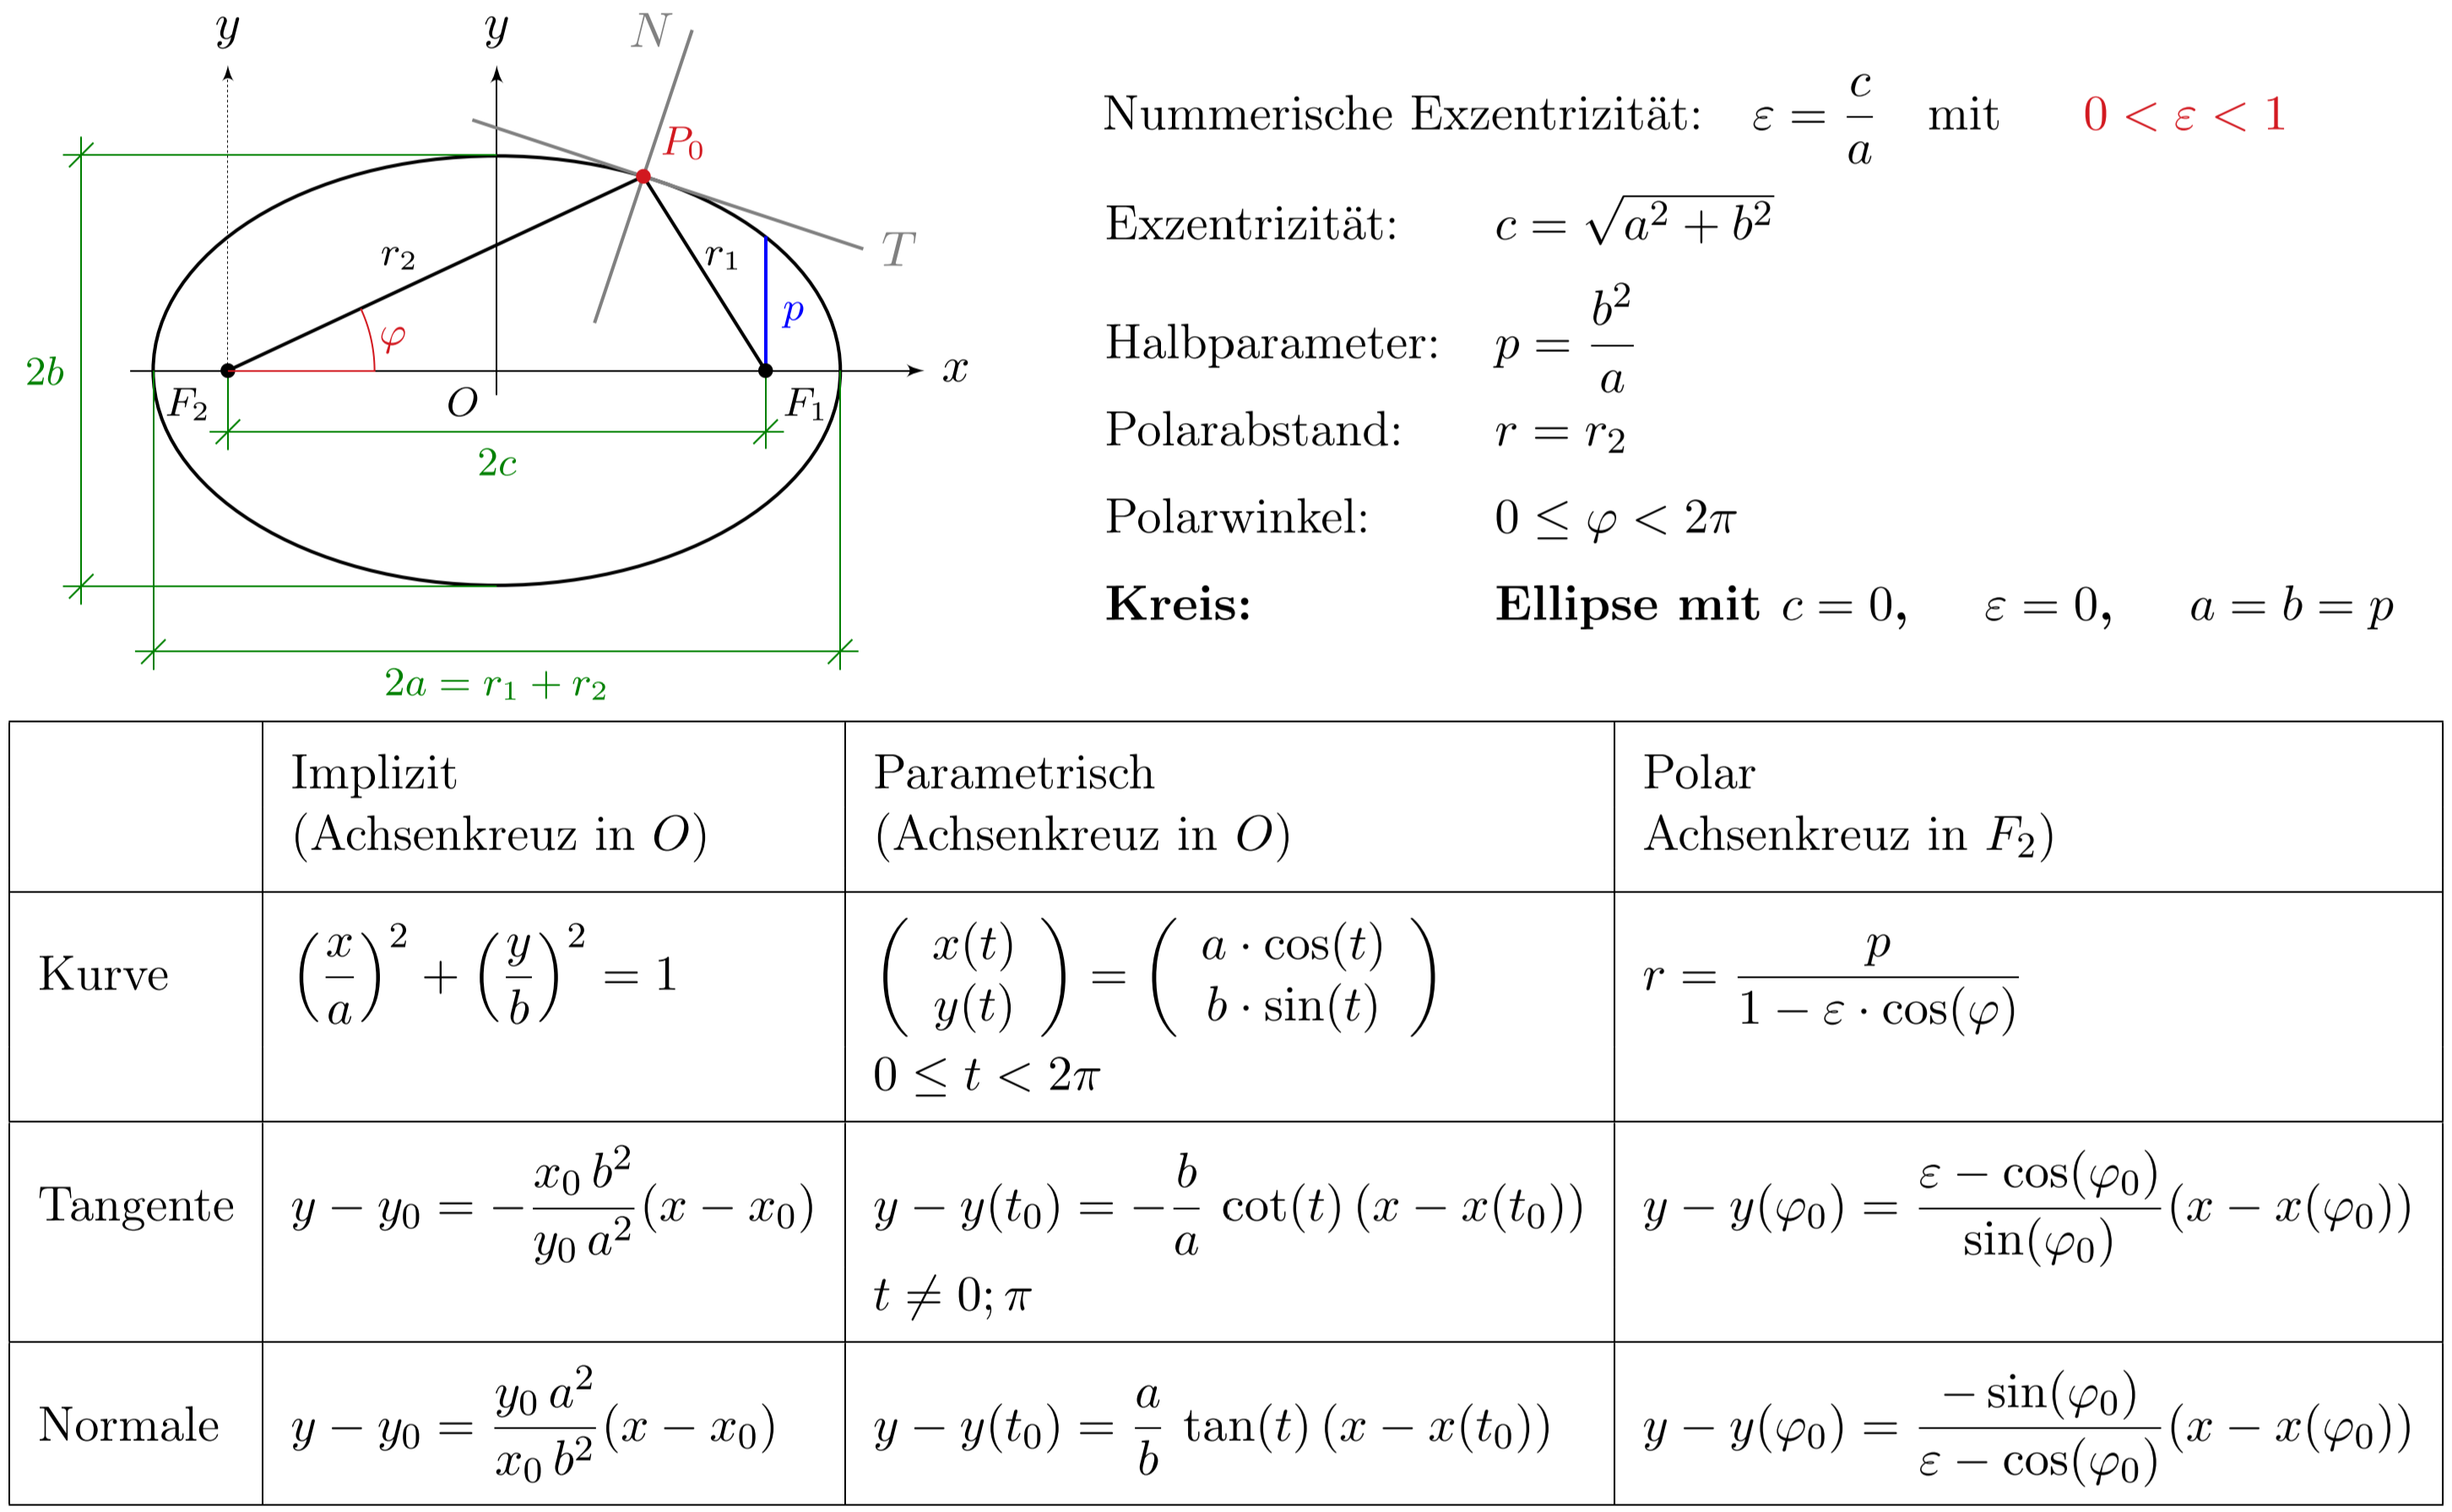
\includegraphics[width=1\textwidth]{bilder/ellipse.png}
	\subsubsection{Kardoide {\formelbuch{100}}} %Seitenzahlen OK 10 Auflage
		\begin{minipage}{.6\textwidth}
			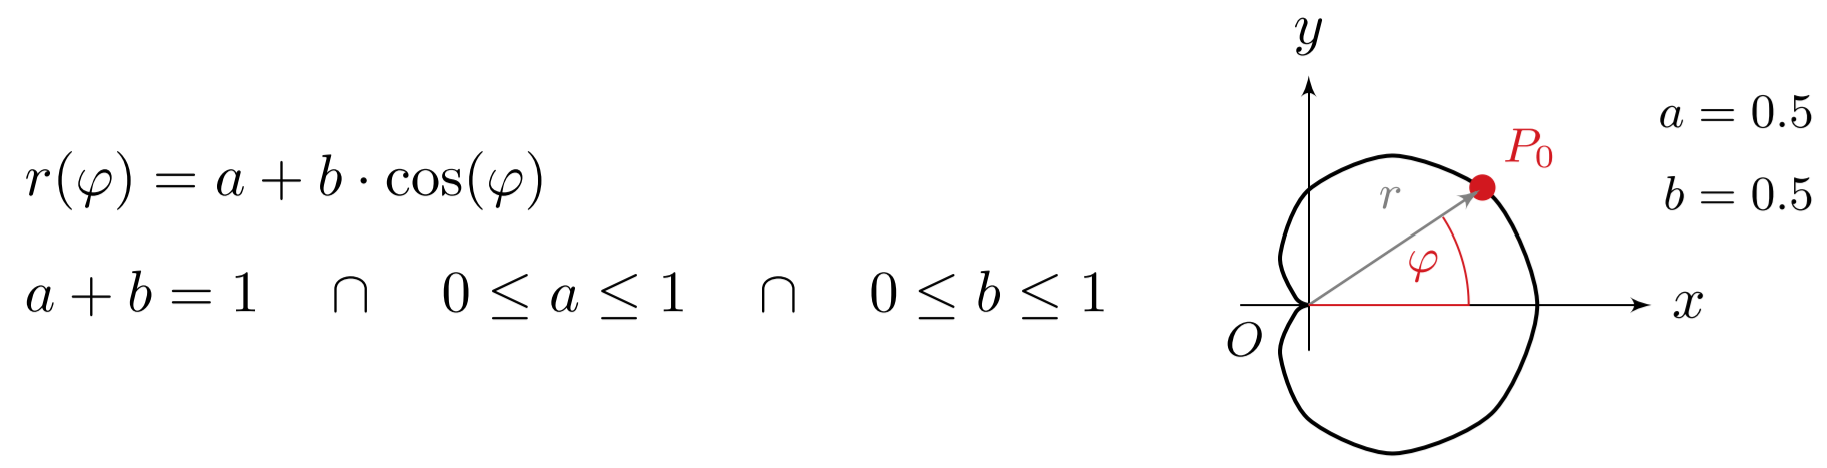
\includegraphics[width=1\textwidth]{bilder/kardoide.png}
		\end{minipage}
		\hspace{5mm}
		\begin{minipage}{.4\textwidth}
			\parbox{2.7cm}{
				\underline{\textbf{Polarform:}} \\
			}
			
			\parbox{5cm}{
				\textbf{Kardioide/Herzk. \formelbuch{100}} \\ %Seitenzahlen OK 10 Auflage
				$r = a(1+\cos(\varphi))$
			}
			
			\parbox{5cm}{
				\textbf{Lemniskate ``$\infty$'' \formelbuch{102}} \\ %Seitenzahlen OK 10 Auflage
				$r = a\sqrt{2\cos(2\varphi)}$ 
			}
			
			\parbox{5cm}{
				\textbf{Strophoide/harm. K. \formelbuch{97}} \\ %Seitenzahlen OK 10 Auflage
				$ r = -a \frac{\cos(2\varphi)}{\cos(\varphi)},(a>0) $ 
			}
		\end{minipage}
	\subsubsection{Parabel {\formelbuch{210}}} %Seitenzahlen OK 10 Auflage
		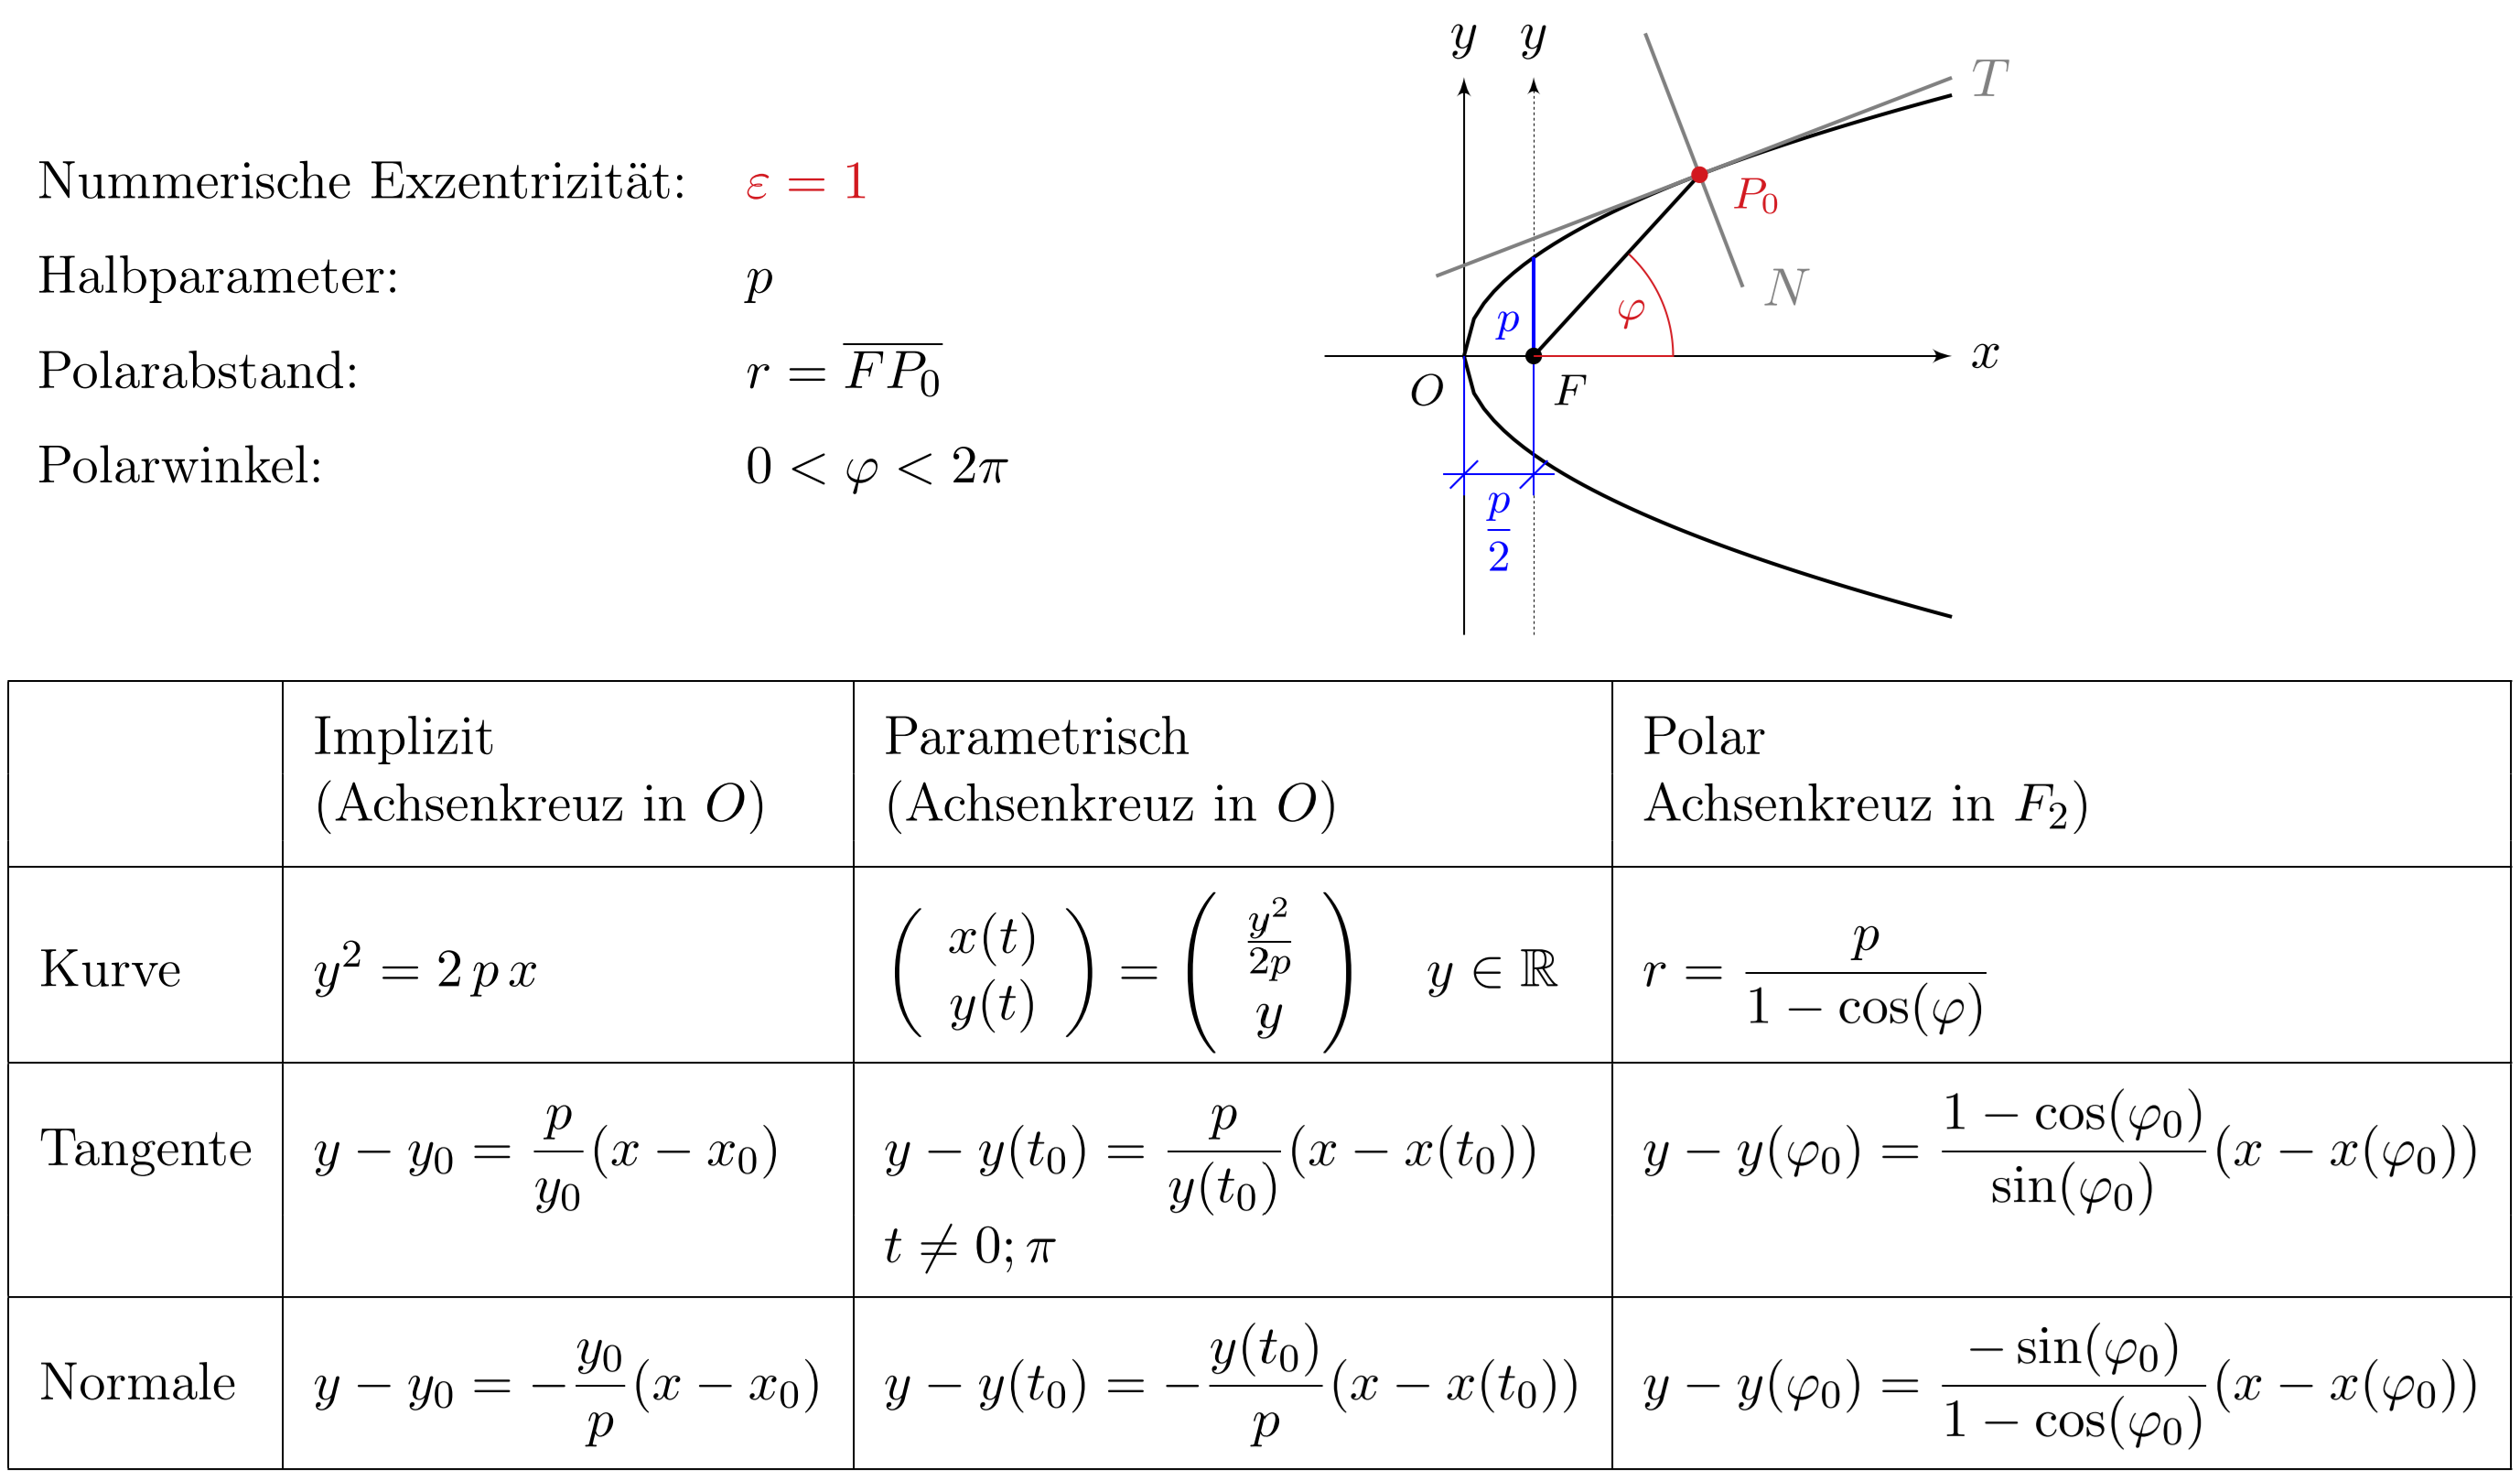
\includegraphics[width=1\textwidth]{bilder/parabel.png}
	\subsubsection{Hyperbel {\formelbuch{207}}} %Seitenzahlen OK 10 Auflage
		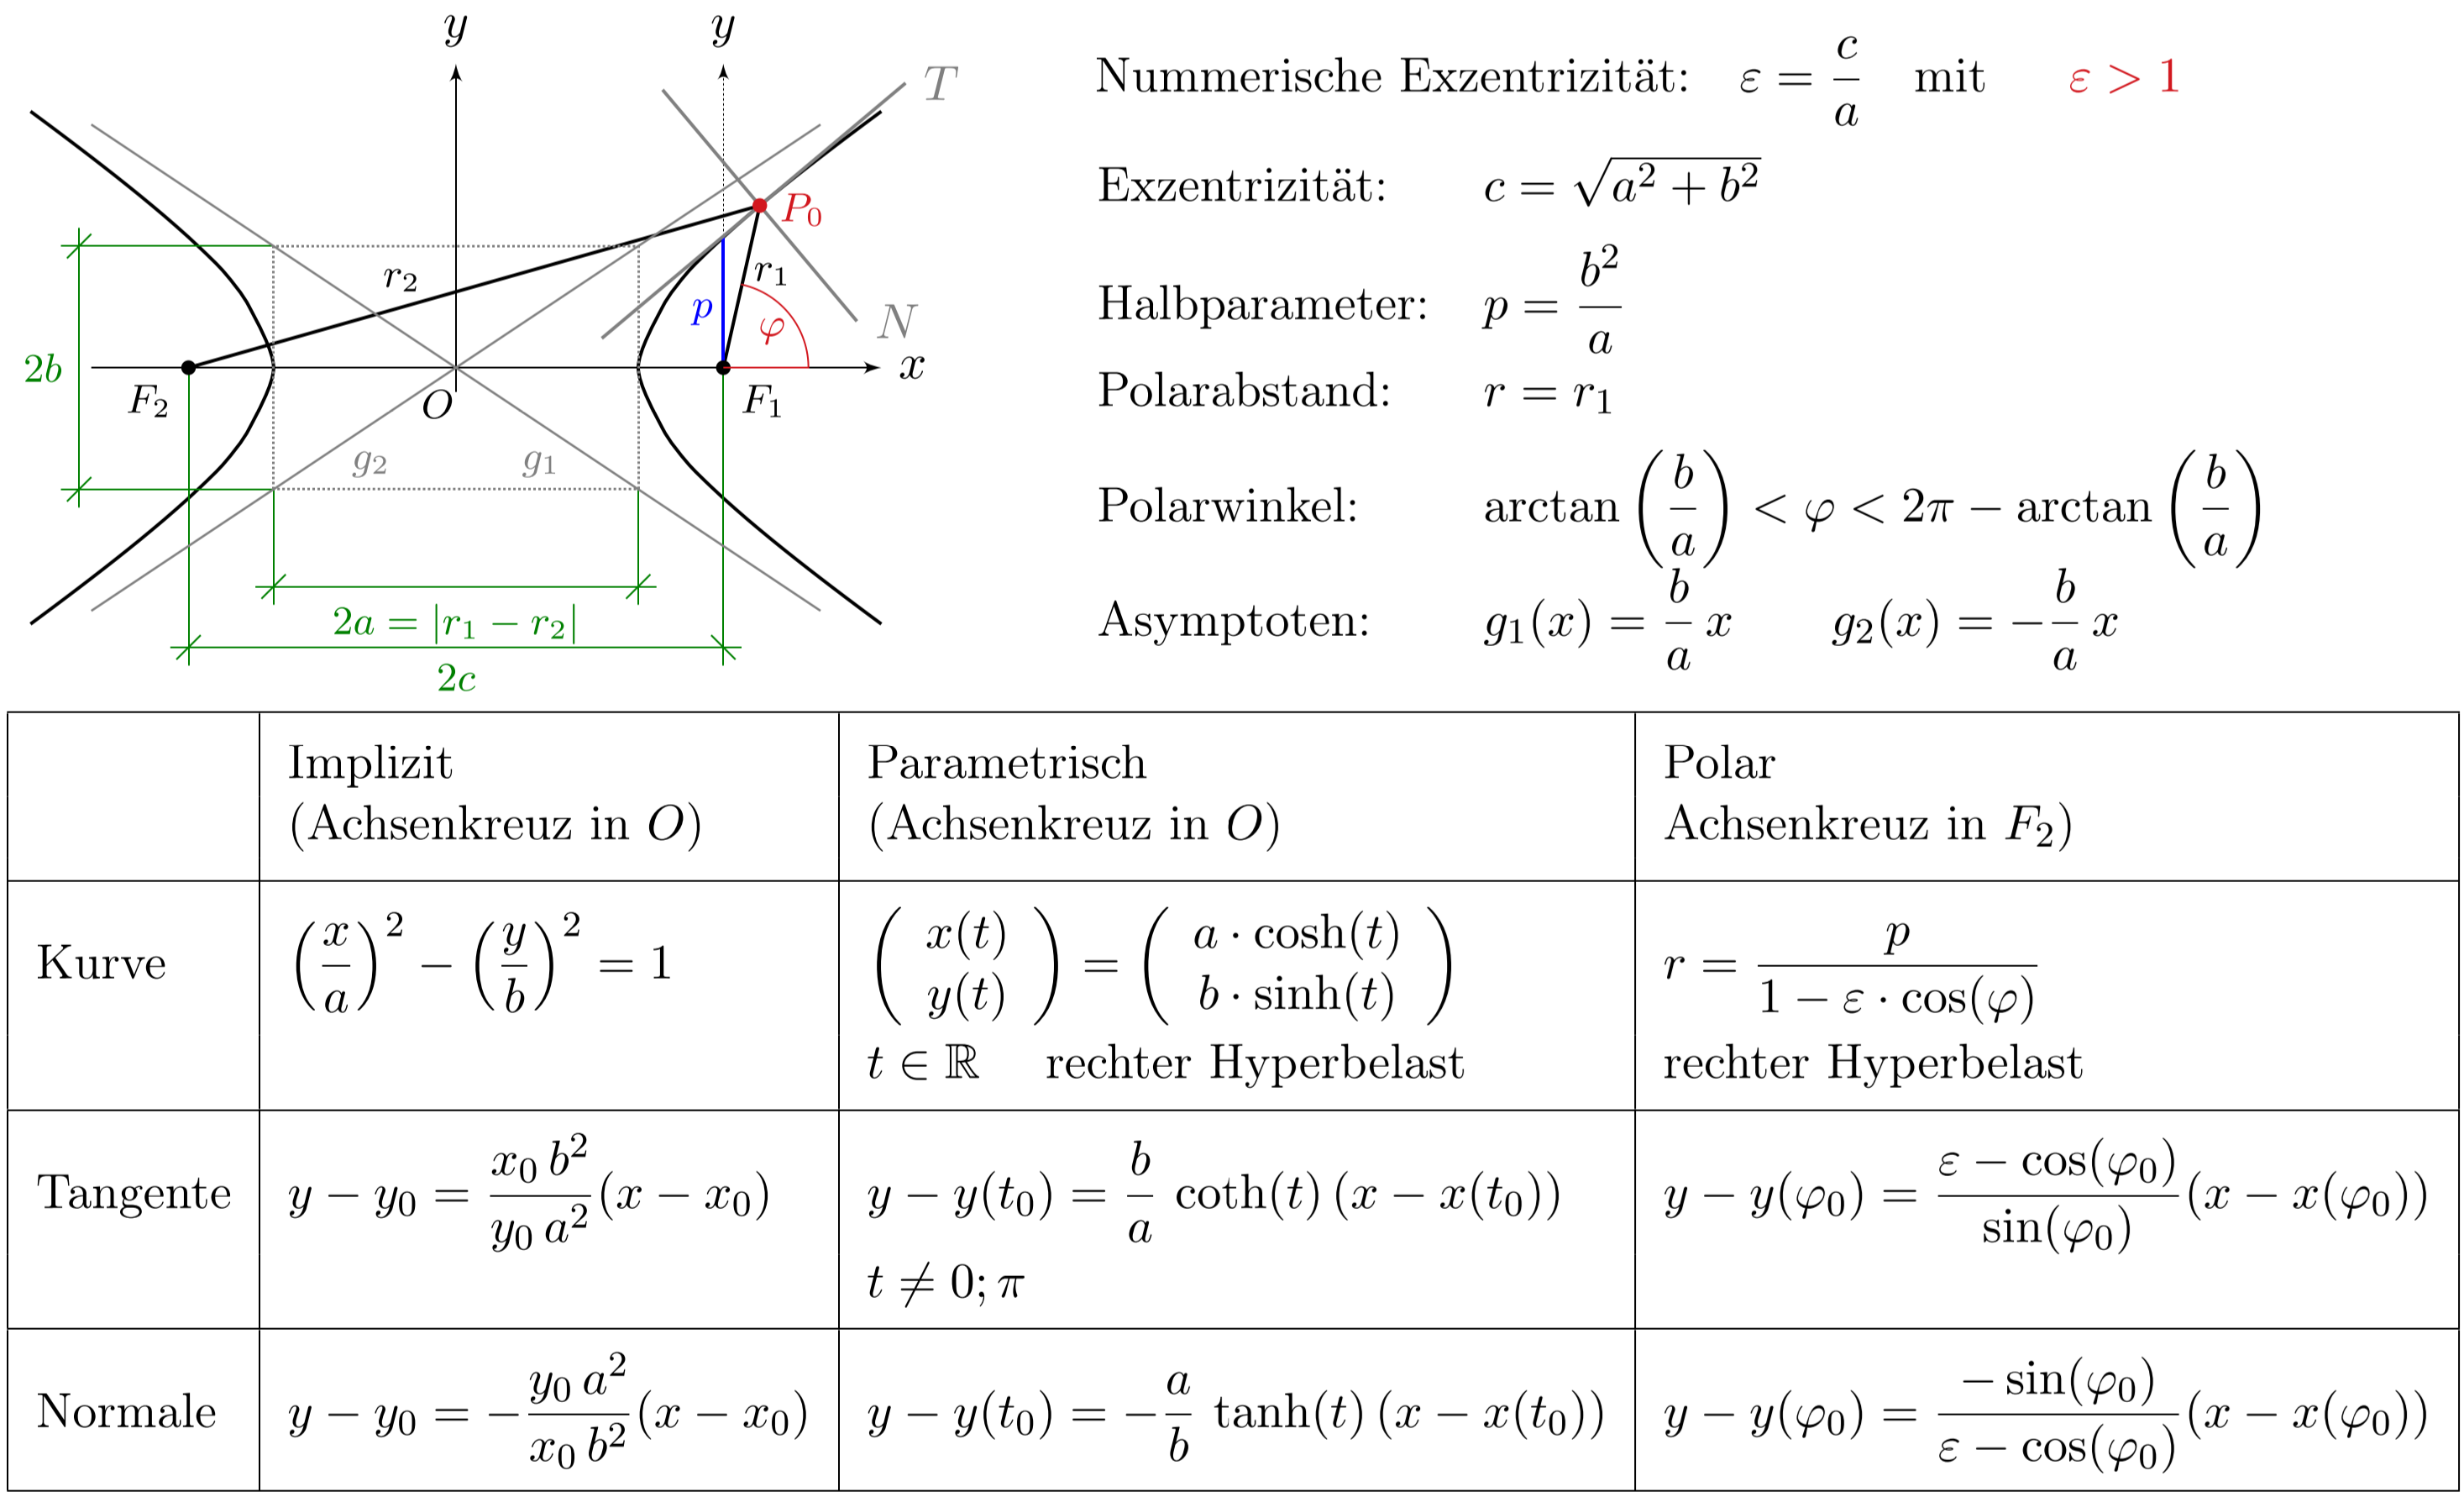
\includegraphics[width=1\textwidth]{bilder/hyperbel.png}


